\documentclass[10pt]{beamer}
\usetheme[
%%% option passed to the outer theme
%    progressstyle=fixedCircCnt,   % fixedCircCnt, movingCircCnt (moving is deault)
  ]{Feather}
  
% If you want to change the colors of the various elements in the theme, edit and uncomment the following lines

% Change the bar colors:
%\setbeamercolor{Feather}{fg=red!20,bg=red}

% Change the color of the structural elements:
%\setbeamercolor{structure}{fg=red}

% Change the frame title text color:
%\setbeamercolor{frametitle}{fg=blue}

% Change the normal text color background:
%\setbeamercolor{normal text}{fg=black,bg=gray!10}

%-------------------------------------------------------
% INCLUDE PACKAGES
%-------------------------------------------------------

\usepackage[utf8]{inputenc}
\usepackage[english]{babel}
\usepackage[T1]{fontenc}
\usepackage{helvet}
\usepackage[T1]{fontenc}
\usepackage{cmap}
\usepackage[utf8]{inputenc}
\usepackage{listings}
\lstset{breakatwhitespace,
language=Matlab,
columns=fullflexible,
keepspaces,
breaklines,
tabsize=3, 
showstringspaces=false,
extendedchars=true}

% DEFFINING AND REDEFINING COMMANDS
%-------------------------------------------------------

% colored hyperlinks
\newcommand{\chref}[2]{
  \href{#1}{{\usebeamercolor[bg]{Feather}#2}}
}

%-------------------------------------------------------
% INFORMATION IN THE TITLE PAGE
%-------------------------------------------------------

\title[] % [] is optional - is placed on the bottom of the sidebar on every slide
{ % is placed on the title page
      \textbf{Hidden Markov Models}
}

\subtitle[Hidden Markov Models]
{
      \textbf{v. 1.1.0}
}

\author[Tien Anh Nguyen]
{      Tien Anh Nguyen \\
      {\ttfamily tien.nguyenanh94@gmail.com}
}

\institute[]
{
      Faculty of Electronics and Computer Engineering\\
      Chonnam National University\\
  
  %there must be an empty line above this line - otherwise some unwanted space is added between the university and the country (I do not know why;( )
}

\date{\today}

%-------------------------------------------------------
% THE BODY OF THE PRESENTATION
%-------------------------------------------------------

\begin{document}

%-------------------------------------------------------
% THE TITLEPAGE
%-------------------------------------------------------

{\1% % this is the name of the PDF file for the background
\begin{frame}[plain,noframenumbering] % the plain option removes the header from the title page, noframenumbering removes the numbering of this frame only
  \titlepage % call the title page information from above
\end{frame}}


\begin{frame}[allowframebreaks]{Content}
\tableofcontents
\end{frame}

%-------------------------------------------------------
\section{References}
%-------------------------------------------------------
\begin{frame}[allowframebreaks]{References}
%-------------------------------------------------------
\begin{thebibliography}{9}
 \bibitem {Richard} Richard A. Davis
  \newblock Introduction to Statistical Analysis of Time Series.
 \bibitem {Brian} Prof. Brian Charles Williams \& Prof. Emillio Frazzoli
  \newblock Principles of Autonomy and Decision Making course. \textcolor{red}{(**)}
  \newblock \emph{MIT OpenCourseWare} 16.410/413, Lecture 20
 \bibitem {Dimitri} Dimitri P. Bertsekas \& John N. Tsitsiklis
  \newblock Introduction to Probability, 2002 \textcolor{red}{(*)}
  \newblock Massachusetts Institute of Technology
  \newblock Department of Electrical Engineering and Computer Science
 \bibitem {Thomas} Thomas Mailund
  \newblock Pattern Recognition In BioInformatics Q3/2012
  \newblock Aarhus University
  \newblock Department of Computer Science
 \bibitem {Anders} Anders Meng
  \newblock An introduction to Markov and Hidden Markov Models \textcolor{red}{(***)}
 \bibitem {Daniel} Daniel Ramage
  \newblock Machine Learning CS229
  \newblock Stanford University
  \newblock December 1, 2007
 \bibitem {UDACITY} Aaron Bobick \& Irfan Essa \& Arpan Chakraborty 
  \newblock Introduction to Computer Vision \textcolor{red}{(**)}
  \newblock UDACITY
  \newblock \emph{https://www.udacity.com/course/ud810}
 \bibitem {Michael} Michael I. Jordan 
  \newblock Practical Machine Learning \textcolor{red}{(*)}
  \newblock University of California, Berkeley
  \newblock \emph{https://people.eecs.berkeley.edu/~jordan/courses/294-fall09/}
 \bibitem {James} Daniel Jurafsky \& James H. Martin 
  \newblock Speech and Language Processing, 2017 \textcolor{red}{(*)}
  \newblock Stanford University
\end{thebibliography}
\end{frame}

%-------------------------------------------------------
\section{Big Picture}
%-------------------------------------------------------
\subsection{Time Series}
\begin{frame}{Big Picture}{Time Series}
%-------------------------------------------------------
  \begin{block}{Time Series}
          Time Series: A collection of observations $q_t$ each one being \
          recorded at time t. (Time could be discrete, t = 1, 2, 3, ..., or \
          continuous t > 0). \cite{Richard}
  \end{block}
\end{frame}

%-------------------------------------------------------
\subsection{Why do we need Markov and Hidden Markov Models?}
%-------------------------------------------------------
\begin{frame}{Big Picture}{iid}
%-------------------------------------------------------
  \begin{itemize}
    \item A model is that observations are assumed to be independent \
          and identically distributed (iid). \cite{Thomas}
  \end{itemize}
  \begin{figure}[h]
    \centering
    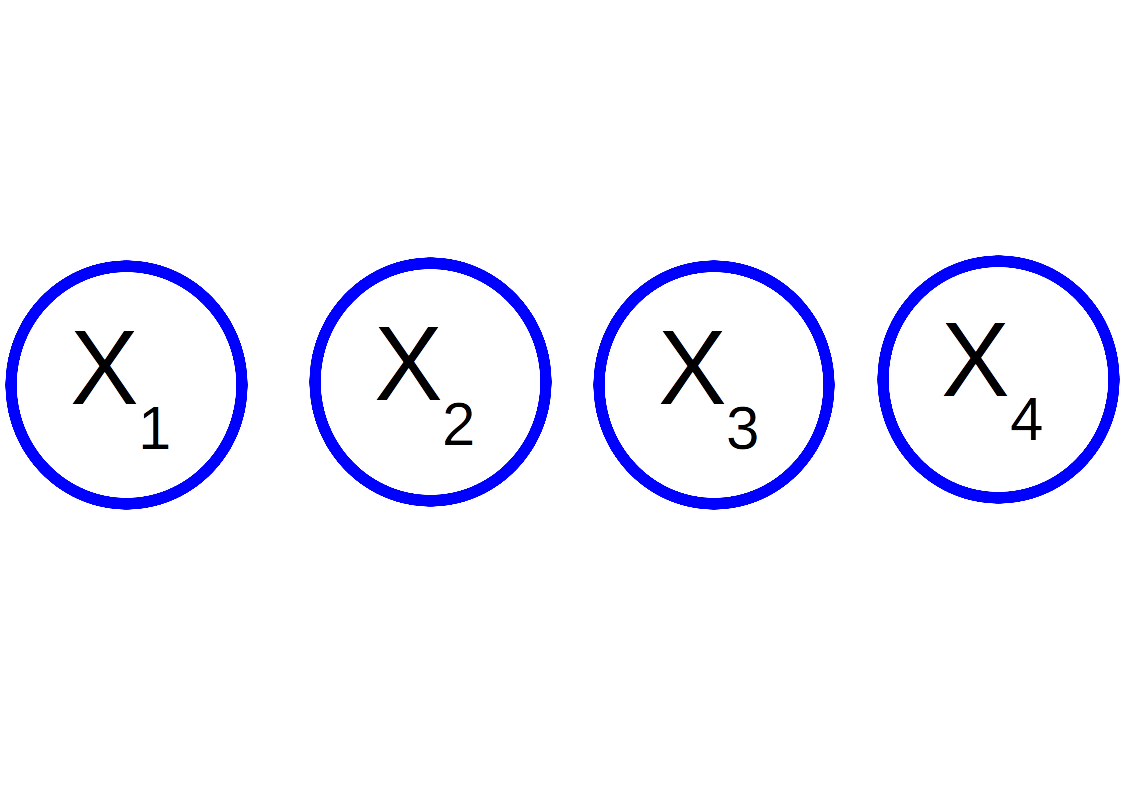
\includegraphics[width=2in,height=2in]{figures/idd.png}
  \end{figure}
\end{frame}

%-------------------------------------------------------
\begin{frame}{Big Picture}{Why do we need Markov and Hidden Markov Models?}
%-------------------------------------------------------
  \begin{itemize}
    \item What are going to happend if observation are dependent?
    \item How can we calculate the "likelihood" of the sample?
  \end{itemize}
  \begin{figure}[h]
    \centering
    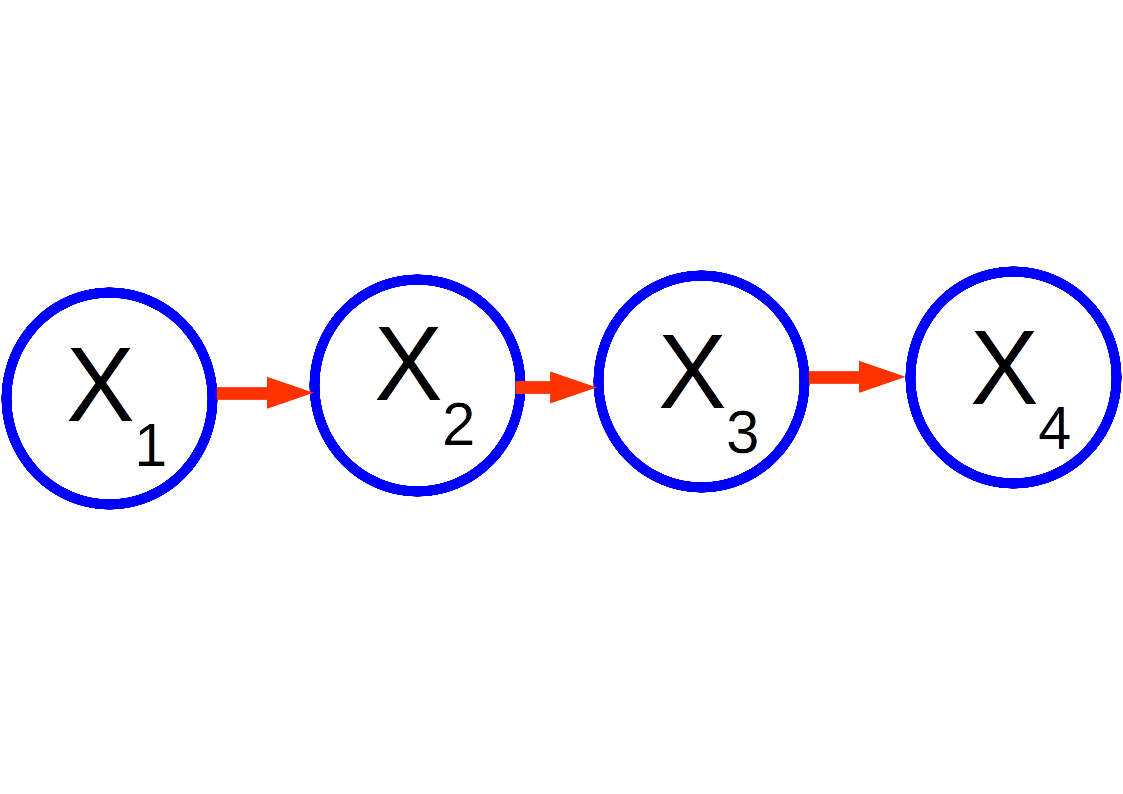
\includegraphics[width=2in,height=1.5in]{figures/not_idd.png}
  \end{figure}
  \begin{itemize}
    \item What will happend if there is a 
          \textcolor{red}{\textbf{time correlation}} between the different\
          samples?\cite{Anders}
  \end{itemize}

\end{frame}

\begin{frame}{Big Picture}{Why do we need Markov Model?}
%-------------------------------------------------------
  \begin{itemize}
    \item How can we predict weather of next day based on weather of today?
  \end{itemize}
  \begin{figure}[h]
    \centering
    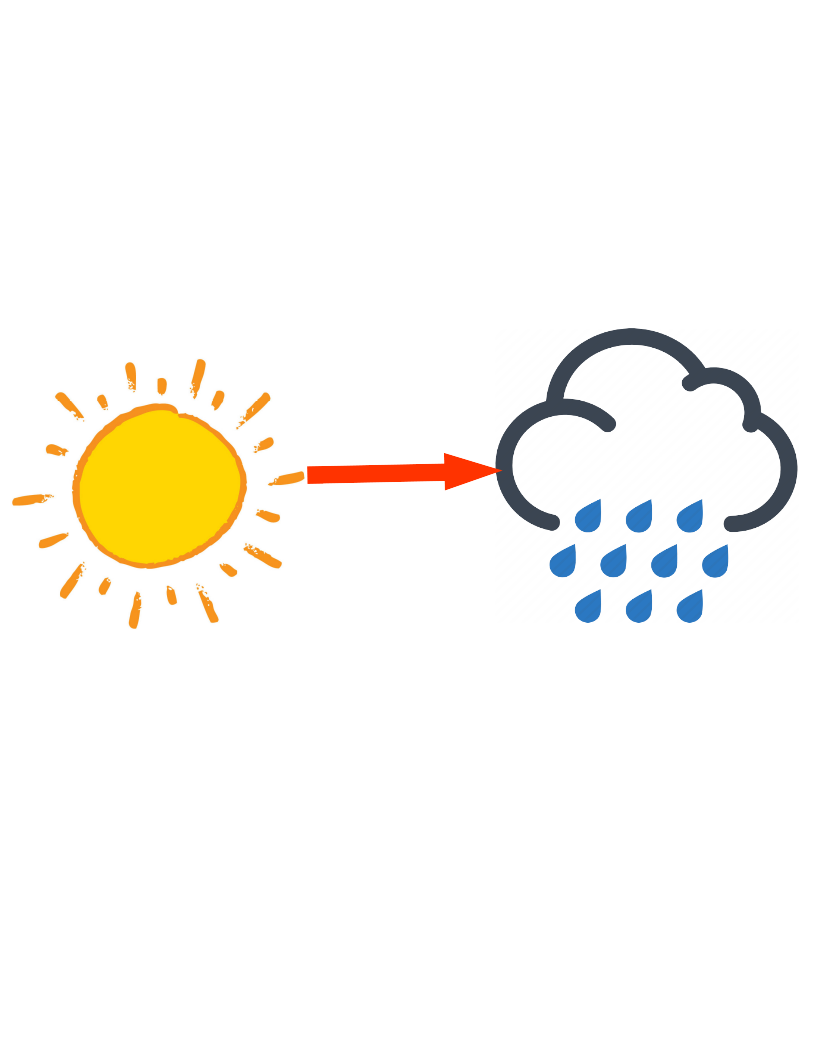
\includegraphics[width=1in,height=1in]{figures/sunny_to_rainny.png}
  \end{figure}
\end{frame}
%-------------------------------------------------------------------------

%-------------------------------------------------------------------------
\begin{frame}{Big Picture}{Why do we need Hidden Markov Models?}
%-------------------------------------------------------
 \label{kidnapping_example}
  \begin{itemize}
    \item Assume that you have been locked into a room for serveral days, \
          and you have no windows, so can we predict the weather outside \
          based on the clothes of the caretaker?\cite{Anders}
  \end{itemize}
  \begin{figure}[h]
    \centering
    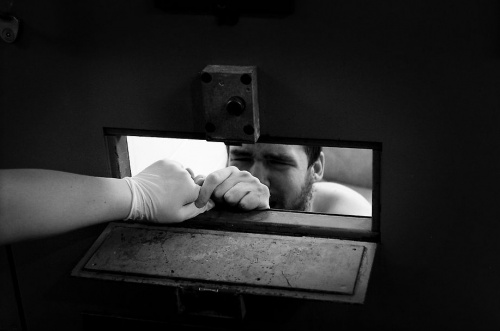
\includegraphics[width=3in,height=2in]{figures/prisoner.jpg}
  \end{figure}
\end{frame}
%-------------------------------------------------------

%-------------------------------------------------------------------------
\begin{frame}{Big Picture}{Why do we need Hidden Markov Models?}
%-------------------------------------------------------
 \label{kidnapping_example}
  \begin{itemize}
    \item On assumption, you are a doctor. There is a patient come to meet you\
          in three days. On the first day, the patient say \textbf{normal}, \
          \text{cold} on the second day and \textbf{dizzy} for the last day. \
          Can we predict the actual state of healthy of the patient on the \
          third day?
  \end{itemize}
  \begin{figure}[h]
    \centering
    
\includegraphics[width=3in,height=2in]{figures/doctor-and-patient.jpg}
  \end{figure}
\end{frame}
%-------------------------------------------------------

%-------------------------------------------------------
\section{Markov Model}
%-------------------------------------------------------
\subsection{Ingredients of a Markov Model}
\begin{frame}{Markov Model}{Ingredients}
  \begin{itemize}
    \item States?
    \item States transition probabilities?
    \item Initial state distribution? 
  \end{itemize}
\end{frame}
%-------------------------------------------------------

%-------------------------------------------------------
\begin{frame}{Markov Model}{Weather Example}
%-------------------------------------------------------
  \begin{block}{Weather Example}
     We have 3 states from a weather system $S = \{Sunny, Rainy, Snowy\}$. We \
     observe the weather a few days \
     $\{q_1 = S_{Sun}, q_2 = S_{Rainy}, q_3 = S_{Snowy}\}$
  \end{block}
  \begin{figure}[h]
    \centering
    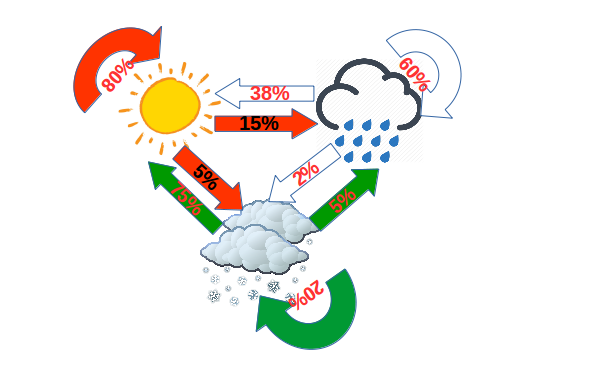
\includegraphics[width=4.5in,height=1.5in]{figures/weather_example.png}
    \caption {Weather: A Markov Model (maybe?)}
  \end{figure}
\end{frame}
%-------------------------------------------------------

%-------------------------------------------------------
\subsection{Markov Assumption}
\begin{frame}{Markov Model}{Markov Assumption}
%-------------------------------------------------------
  \begin{block}{FIRST ORDER MARKOV ASSUMPTION}
        The probability of being in a state at time $t+1$ depends only on the\
        state at time $t$. It means that the state at time $t$ represents\
        "enough" summary of the past to reasonably predict the feature\cite{Daniel}. 
        Formally:\\
        \begin{equation}
            P(q_t|q_{t-1},...,q_1) = P(q_t|q_{t-1})
        \end{equation}
  \end{block}
  \begin{block}{STATIONARY PROCESS ASSUMPTION}
       The conditional distribution over next state given current state does \
       not change over time\cite{Daniel}. Formally:\\
        \begin{equation}
             P(q_t|q_{t-1}) = P(q_2|q_1);t \in 2..T
        \end{equation}
  \end{block}
  \textit{What is the meaning of the \textbf{Stationary Process Assumption}?}\\
  We are going to get back this assumption later!!!!!!!!
\end{frame}
%-------------------------------------------------------

%-------------------------------------------------------
\subsection{Definition}
\begin{frame}{Markov Model}{DEFINITION}
%-------------------------------------------------------
  \begin{block}{Definition(Markov Model)}
     A Markov model (Markov Chain) is a sequence of random variables \ 
     $q_1,\ q_2,\ q_3,\ ...,\ q_N$, such that the probability\
     distribution of $q_{t+1}$ depends only on the outcome at $q_t$.
  \end{block}
\end{frame}
%-------------------------------------------------------

%-------------------------------------------------------
\subsection{Likelihood Calculation}
\begin{frame}{Markov Model}{Likelihood Calculation}
%-------------------------------------------------------
  \begin{block}{Likelihood Calculation}
  We assump that there are a given sequence of data $Q=\{q_1, q_2, ..., q_N\}$ \
  where each of the variables $q_n$ take one of \textbf{S} states $\{S_1, S_2, ..., S_{|S|}\}$.
  The likelihood of the sample \textbf{D} can now be calculated as:\\
        \begin{equation}
            P(Q|M) = P(q_1 = S_i)\displaystyle \prod_{n=2}^{N}p(q_n = S_j | q_{n-1} = S_i)
        \end{equation}
  \end{block}
\end{frame}
%-------------------------------------------------------

%-------------------------------------------------------
\begin{frame}{Markov Model}{Likelihood Calculation}
  \begin{itemize}
    \item The conditional probabilities $P(x_n = S_j | x_{n-1} = S_i)$ are \
          referred to as \textbf{state transition probabilities} or simple \
          \textbf{transition probabilities}. \cite{Anders}
    \item In most cases we assume that the \textit{transition probabilities} \
          are homogeneous, which means that the probabilities do not change \
          over time(STATIONARY PROCESS ASSUMPTION). \cite{Anders} Formally:
          \begin{equation}
               P(x_n = S_j|x_{n-1} = S_i) = P(x_{n+T} = S_j|x_{n-1+T} = S_i)
          \end{equation}
          Where T is a positive integer larger or equal to one.
  \end{itemize}
\end{frame}
%-------------------------------------------------------

%-------------------------------------------------------
\subsection{Transition Matrix}
\begin{frame}{Markov Model}{Transition Matrix}
%-------------------------------------------------------
  \begin{block}{Transition Matrix}
  The transition probabilites can be written as a transition matrix, which is \
  of dimension $M\ x\ M$. Since each element in the matrix represent a\
  probability of staying or jumping to another state. \cite{Anders}
        \begin{equation}
            A = 
            \begin{bmatrix}
                a_{11} & a_{12} & a_{13}\\
                a_{21} & a_{22} & a_{23}\\
                a_{31} & a_{32} & a_{33}\\
            \end{bmatrix}
        \end{equation}
  \end{block}
  \begin{itemize}
      \item Each entry must be positive, so $a_{ij} \geqslant 0$ for all i,j.
      \item Each row must sum up to one, since each row represents the\
            probability of jumping from or staying in the state. Formally: \\
            \begin{equation}
               \sum_{j=1}^{M}a_{ij} = 1\ for\ i\ =\ 1\ ...\ M
            \end{equation} 
  \end{itemize}
\end{frame}
%-------------------------------------------------------

%-------------------------------------------------------
\subsection{Illustration of the Markov Model}
\begin{frame}{Markov Model}{Illustration}
%-------------------------------------------------------
  \begin{figure}[h]
    \centering
    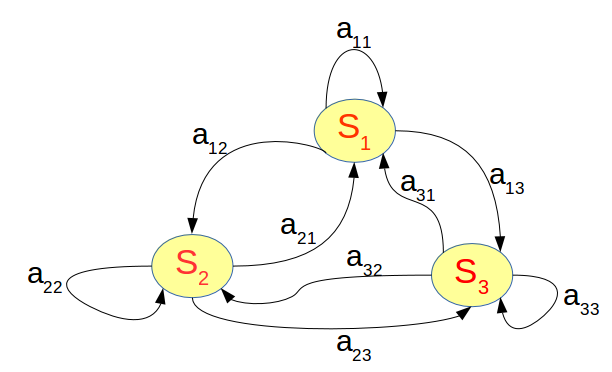
\includegraphics[width=4.5in,height=2.3in]{figures/illustration_markov_model.png}
    \caption {\textbf{Illustration of the Markov Model}}
  \end{figure}
\end{frame}
%-------------------------------------------------------

%-------------------------------------------------------
\begin{frame}{Markov Model}{Graphical Models}
%-------------------------------------------------------
  \begin{itemize}
      \item There is no time information in the illustration.
  \end{itemize}
\end{frame}
%-------------------------------------------------------

%-------------------------------------------------------
\subsection{Illustration of the Markov Model}
\begin{frame}{Markov Model}{Graphical Model}
%-------------------------------------------------------
  \begin{figure}[h]
    \centering
    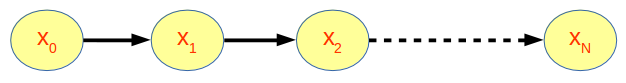
\includegraphics[width=2.5in,height=1in]{figures/graphical_models.png}
    \caption {\textbf{Graphical model of Markov Model}}
  \end{figure}
\end{frame}
%-------------------------------------------------------

%-------------------------------------------------------
\subsection{Initial State Probability}
\begin{frame}{Markov Model}{Graphical Model}
%-------------------------------------------------------
  \begin{block}{Intial State Probability}
   To fully characterize the Markov Model, we need to address the 
   \textbf{initial state probability} which is given as \
   $\pi_i$. $\pi_i$ is the probability that the Markov chain will start in\
   state i.\\
        \begin{equation}
            \pi = \pi_1, \pi_2,...,\pi_N
        \end{equation}
        \begin{equation}
           \sum_{i=1}^{N}\pi_i = 1 
        \end{equation}
  \end{block}
\end{frame}
%-------------------------------------------------------

%-------------------------------------------------------
\subsection{Weather Example cont.}
\begin{frame}[allowframebreaks]{Markov Model}{Weather example cont.}
%-------------------------------------------------------
That is enough for theory. Let go back to \textbf{Weather Example}. 
  \begin{figure}[h]
    \centering
    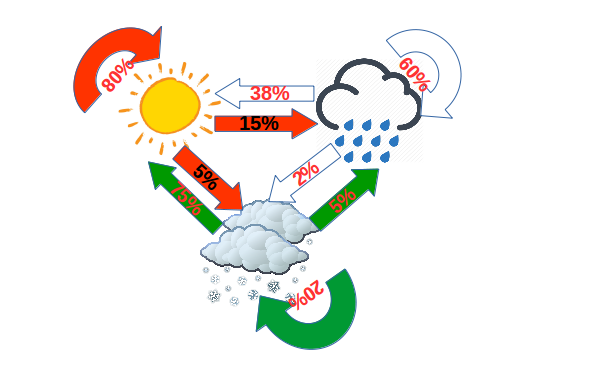
\includegraphics[width=4.6in,height=2.3in]{figures/weather_example.png}
    \caption {\textbf{Weather?A Markov Model?}}
  \end{figure}
  \textbf{Ingredients of a Markov Model}
  \begin{itemize}
      \item States: $\{S_{Sunny},\ S_{rainy},\ S_{snowy}\}$
      \item State transition probabilities:
            \begin{center}
              \begin{tabular}{ |p{2cm}|p{1.2cm}|p{1.2cm}|p{1.2cm}| }
                \hline
                 \multicolumn{4}{|c|}{Weather Markov Model} \\
                \hline
                        & Sunny & Rainy & Snowy \\
                \hline
                     Sunny & 0.8  & 0.15 & 0.05\\
                     Rainy & 0.38 & 0.6  & 0.02\\
                     Snowy & 0.75 & 0.05 & 0.2\\
                \hline
              \end{tabular}
              \end{center}
      \item On assumption, initial state distribution: $\pi = (0.7\ \ 0.25\ \ 0.05)$
  \end{itemize}
  \begin{figure}[h]
    \centering
    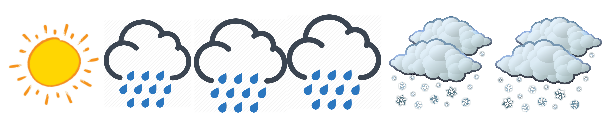
\includegraphics[width=3.5in,height=1.5in]{figures/weather_example_2.png}
    \caption {\textbf{What is the probability of this series?}}
  \end{figure}
   \begin{block}{Solution}
       \fontsize{7}{10}{$P(S_{sunny}).P(S_{rainy}|S_{sunny}).P(S_{rainy}|S_{rainy}).P(S_{rainy}|S_{rainy})$}\
       $.P(S_{snowy}|S_{rainy}).P(S_{snowy}|S_{snowy})$\\
       $=0.7\cdot0.15\cdot0.6\cdot0.6\cdot0.02\cdot0.2=0.0001512$
   \end{block}
\end{frame}
%-------------------------------------------------------

%-------------------------------------------------------
\section{Hidden Markov Model}
%-------------------------------------------------------
\subsection{Kidnapping Example}
\begin{frame}{Hidden Markov Model}{Kidnapping Example}
    Let go back to \hyperlink{kidnapping_example}{\beamerbutton{\textbf{Kidnapping Example}}}
\end{frame}
%-------------------------------------------------------

%-------------------------------------------------------
\subsection{Kidnapping vs Weather Example}
%-------------------------------------------------------
\begin{frame}{Hidden Markov Model}{Kidnapping vs Weather Example}
%-------------------------------------------------------
   \begin{block}{Kidnapping Example vs Weather Example}
     What does \textbf{Kidnapping} example different from \textbf{Weather} example?
   \end{block}
\end{frame}
%-------------------------------------------------------

%-------------------------------------------------------
\begin{frame}{Hidden Markov Model}{Kidnapping vs Weather Example cont.}
%-------------------------------------------------------
   \begin{block}{Kidnapping Example vs Weather Example cont.}
     In the \textbf{Kidnapping} example, we cannot directly observe the\
     \textbf{S} states {$\{S_{Sunny},\ S_{rainy},\ S_{snowy}\}$}. They are\
     now \textbf{hidden state variables}.
   \end{block}
\end{frame}
%-------------------------------------------------------

%-------------------------------------------------------
\subsection{Hidden State Variables}
%-------------------------------------------------------
\begin{frame}[allowframebreaks]{Hidden Markov Model}{Hidden State Variables}
   \begin{block}{Hidden Variables}
       The hidden state variables are observed through another variable $O$,\
       which gives an indication of the hidden state\cite{Anders}.
       The observed variable $O$ can be discrete or continuous random varibale.
   \end{block}
   \begin{block}{The relationship between $O$ and $Q$}
        Assume that the observable's are discrete taking on one of L values \
        $\{C_1, C_2,...,C_{|L|}\}$. Hence, we have the relationship between the\
       \textbf{ observed variables $Q$} and \textbf{hidden state variables $O$}. \
       Formally:\\
             \begin{equation}
             \label{rela_M_Y}
                  P(o_n = C_i|q_n = S_j) = b_{i,j}
             \end{equation}
   \end{block}
%-------------------------------------------------------
\end{frame}
%-------------------------------------------------------

%-------------------------------------------------------
\subsection{Emission Probability}
%-------------------------------------------------------
\begin{frame}{Hidden Markov Model}{Emission Probability}
   \begin{block}{Emission Probability}
        The equation [\ref{rela_M_Y}] means that given we are in state $S_j$ of \
        hidden variable at some time instant n, what is the probability of\ 
        observing the symbol $C_j$
   \end{block}
   \begin{block}{Emission Probability}
        The output of the expression [\ref{rela_M_Y}] is called\
        \textbf{emission probability}
   \end{block}
   \begin{block}{Emission Probability Matrix}
        The output of the expression [\ref{rela_M_Y}] can be fully described by \
        a $LxM$ emission (observation) matrix \textbf{B}.
   \end{block}
%-------------------------------------------------------
\end{frame}
%-------------------------------------------------------

%-------------------------------------------------------
\subsection{Graphical Model of a Hidden Markov Model}
%-------------------------------------------------------
\begin{frame}{Hidden Markov Model}{Graphical Model of a Hidden Markov Model}
%-------------------------------------------------------
  \begin{figure}[h]
    \centering
    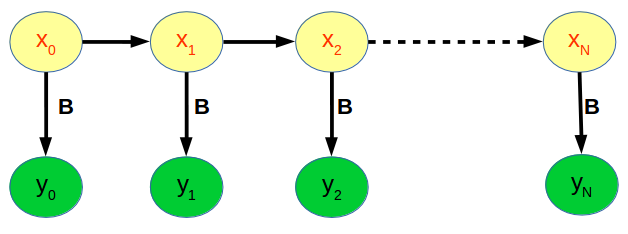
\includegraphics[width=3.5in,height=2in]{figures/graphical_model_hidden_markov_model.png}
    \caption {\textbf{Graphical model of a Hidden Markov Model}}
  \end{figure}
\end{frame}
%-------------------------------------------------------

%-------------------------------------------------------
\subsection{Three Fundamental Problems of Hidden Markov Model}
%-------------------------------------------------------
\begin{frame}{Hidden Markov Model}{Three Fundamental Problems of Hidden Markov Model}
   \begin{block}{Likelihood}
       Given a HMM $\lambda=(A,B)$ and an observation sequence $O$, determine\
       the likelihood $P(O|\lambda)$.
   \end{block}
   \begin{block}{Decoding}
       Given a HMM $\lambda=(A,B)$ and an observation sequence $O$, discover\
       the best hidden state sequence $Q$.
   \end{block}
   \begin{block}{Learning}
       Given an observation sequence $O$ and the set of states in the HMM, \
       learn the HMM parameters A and B.
   \end{block}
%-------------------------------------------------------
\end{frame}
%-------------------------------------------------------

%-------------------------------------------------------
\subsection{Likelihood Computation: The Forward ALgorithm}
%-------------------------------------------------------
\begin{frame}{Hidden Markov Model}{Likelihood Computation: The Forward ALgorithm}
   \begin{block}{Likelihood}
       Given a HMM $\lambda=(A,B)$ and an observation sequence $O$, determine\
       the likelihood $P(O|\lambda)$.
   \end{block}
   To calculate the probability of a serie of the hidden events is not so \
   so simple in Hidden Markov models. Therefore, let's start with a slightly \
   simple situation \textbf{Eating Ice Cream}.

%   \begin{block}{Likelihood Computation: The Forward ALgorithm}
%        To calculate the likelihood of the set of observations \
%        $Y=\{y_1,\ y_2,\ ...,\ y_N\}$ using the following formula:
%             \begin{equation}
%             \label{hidd_likelihood}
%                  P(D) = \sum_{n=1}^{N}P(x_1)p(y_1|x_1)\prod_{n=2}^{N}P(x_n|x_{n-1})P(y_n|x_n)
%             \end{equation}
%   \end{block}
%   \begin{block}{The likelihood and transition matrix}
%        The expression [\ref{hidd_likelihood}] can be rewrite using the notation \
%        of transition matrix, observation matrix and initial state probability.
%             \begin{equation}
%             \label{hidd_likelihood}
%                  P(D) = \sum_{x_1,x_2,...,x_n}^{}\pi_{x_1}(1)b_{x_1}(y_1)\prod_{n=2}^{N}a_{x_{n-1},x_n}b_{x_n}(y_n)
%             \end{equation}
%        where $b_{x_n} = S_j(y_n = C_i) = b_{j,i}$ is the emission probability.
%   \end{block}
%-------------------------------------------------------
\end{frame}
%-------------------------------------------------------

%-------------------------------------------------------
\begin{frame}{Hidden Markov Model}{Eating Ice Creams Example}
%-------------------------------------------------------
   Imagine that you are a climatologist in the year 2799 studying the history\
   of global warming. You cannot find any records of the weather in Baltimore,\
   Maryland, for the summer of 2007, but you do find Jason Eisner’s diary,\
   which lists how many ice creams Jason ate every day that summer. Our goal\
   is to use these observations to estimate the temperature every day. We’ll\
   simplify this weather task by assuming there are only two kinds of days:\
   cold (C) and hot (H).

   \begin{block}{Eating Ice Creams Example}
       Given a sequence of observations O, each observation is an integer\
       corresponding to the number of ice creams eaten on a given day, figure\
       out the correct ‘hidden’ sequence Q of weather states (H or C) which\ 
       caused Jason to eat the ice cream.
   \end{block}
%-------------------------------------------------------
\end{frame}
%-------------------------------------------------------

%-------------------------------------------------------
\begin{frame}{Hidden Markov Model}{Likelihood Computation: The Forward ALgorithm}
%-------------------------------------------------------
   \begin{block}{The likelihood of the observation sequence}
        Each hidden state produces only a single observation. Thus, the\
        sequence of hidden states and the sequence of observations have\
        the \textbf{same length T}. Given a particular hidden state sequence\
        $Q=\{q_0, q_1, q_2, ..., q_T\}$ and an observation sequence\
        $O=\{o_1, o_2, ..., o_T\}$, the likelihood of the observation sequence\
        is:
             \begin{equation}
             \label{likelihood_compute_1}
                  P(O|Q) = \prod_{i=1}^{T}P(o_i|q_i)
             \end{equation}
   \end{block}
%-------------------------------------------------------
\end{frame}
%-------------------------------------------------------

%-------------------------------------------------------
\begin{frame}{Hidden Markov Model}{Likelihood Computation: The Forward ALgorithm}
%-------------------------------------------------------
   \begin{block}{Eating Ice Creams Example}
         Let make the example more simpler. Suppose that we already knew the \
         weather and want to predict how much ice cream Jason would eat. Let \
         compute the probability of ice-cream observation \textit{3 1 3} from\
         one possible hidden state sequence \textit{hot hot code}\\
         $P(3\ 1\ 3|hot\ hot\ cold) = P(3|hot) \cdot P(1|hot| \cdot P(3|cold)$
   \end{block}
  \begin{figure}[h]
    \centering
    
\includegraphics[width=4in,height=1in]{figures/ice_creams_example_01.png}
    \caption {\textbf{The computation of the observation likelihood}}
  \end{figure}
%-------------------------------------------------------
\end{frame}
%-------------------------------------------------------

%-------------------------------------------------------
\begin{frame}{Hidden Markov Model}{Likelihood Computation: The Forward ALgorithm}
%-------------------------------------------------------
      \textcolor{red}{If we don't actually know what the hidden state\
                 (weather) sequence was?}
%-------------------------------------------------------
\end{frame}
%-------------------------------------------------------

%-------------------------------------------------------
\begin{frame}{Hidden Markov Model}{Likelihood Computation: The Forward ALgorithm}
%-------------------------------------------------------
   \begin{block}{Likelihood Computation}
       We can compute the total probability of the observation just by\
       summing over all possible hidden state sequences:
          \begin{equation}
            P(O) = \sum_{Q}^{}P(O, Q) = \sum_{Q}^{}P(O|Q)P(Q)
          \end{equation}
   \end{block}
%-------------------------------------------------------
\end{frame}
%-------------------------------------------------------

%-------------------------------------------------------
\begin{frame}{Hidden Markov Model}{Likelihood Computation: The Forward ALgorithm}
%-------------------------------------------------------
   \begin{block}{Eating Ice Creams Example}
         $P(3\ 1\ 3) = P(3\ 1\ 3, cold\ cold\ cold) + P(3\ 1\ 3, cold\ cold\ hot) + ...$
   \end{block}
%-------------------------------------------------------
\end{frame}
%-------------------------------------------------------

%-------------------------------------------------------
\begin{frame}{Hidden Markov Model}{Likelihood Computation: The Forward ALgorithm}
%-------------------------------------------------------
   \begin{block}{Likelihood Computation}
        For an HMM with N hidden states and an observation sequence of T \
        observations, there are $N^{T}$ possible hidden sequences. For a \
        real tasks, where N and T are both large, $N^{T}$ is a very large \
        number, so we cannot compute the total observation likelihood by \
        computing a separate observation likelihood for each hidden state \
        sequence and then summing them. \textbf{The Forward algorithm is a\
        solution for that problem}.
   \end{block}
%-------------------------------------------------------
\end{frame}
%-------------------------------------------------------

%-------------------------------------------------------
\begin{frame}{Hidden Markov Model}{Likelihood Computation: The Forward ALgorithm}
%-------------------------------------------------------
  \begin{figure}[h]
    \centering
    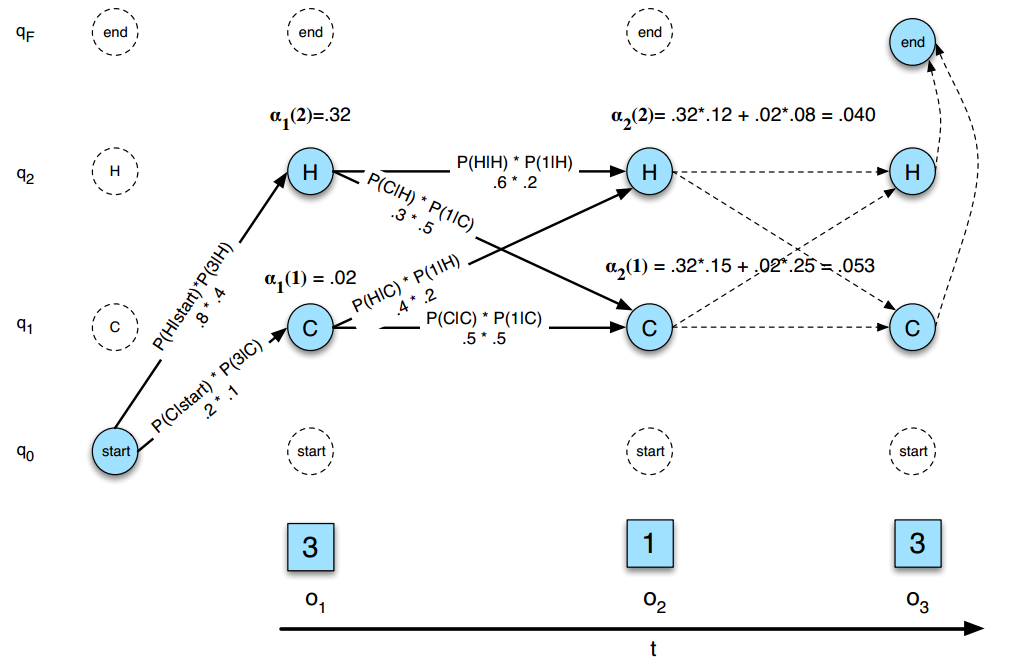
\includegraphics[width=4in,height=2.3in]{figures/the_forward_trellis.png}
    \caption {\textbf{The forward trellis}}
  \end{figure}
%-------------------------------------------------------
\end{frame}
%-------------------------------------------------------

%-------------------------------------------------------
\begin{frame}{Hidden Markov Model}{Likelihood Computation: The Forward ALgorithm}
%-------------------------------------------------------
    \begin{itemize}
      \item \textcolor{red}{What is the Forward algorithm?}
    \end{itemize}
%-------------------------------------------------------
\end{frame}
%-------------------------------------------------------

%-------------------------------------------------------
\begin{frame}{Hidden Markov Model}{Likelihood Computation: The Forward Algorithm}
%-------------------------------------------------------
    \begin{block}{The Forward Algorithm}
        The forward algorithm computes the observation probability by summing\
        over the probabilities of all possible hidden state paths that could\  
        generate the observation sequence, but it does so efficiently by\
        implicitly folding each of these paths into a single forward trellis.
    \end{block}
%-------------------------------------------------------
\end{frame}
%-------------------------------------------------------

%-------------------------------------------------------
\begin{frame}{Hidden Markov Model}{Likelihood Computation: The Forward Algorithm}
%-------------------------------------------------------
    \begin{block}{Cells of the Forward algorithm trellis}
         Each cell of the forward algorithm trellis $\alpha_t(j)$ represents\
         the probability of being in state $j$ after seeing the first $t$\
         observations, given the automaton $\lambda$.
    \end{block}
    \begin{block}{Cells of the Forward algorithm trellis}
         The value of each cell $\alpha_t(j)$ is computed by summing over the\
         probabilities of every path that could lead us to this cell.
    \end{block}
%-------------------------------------------------------
\end{frame}
%-------------------------------------------------------

%-------------------------------------------------------
\begin{frame}{Hidden Markov Model}{Likelihood Computation: The Forward Algorithm}
%-------------------------------------------------------
    \begin{block}{Cells of the Forward algorithm trellis}
        \begin{equation}
            \alpha_t(j) = P(o_1, o_2, ..., o_t, q_t = j|\lambda) = \sum_{i=1}^{N}\alpha_{t-1}(i)a_{ij}b_j(o_t)
        \end{equation}
    \end{block}
    \begin{itemize}
        \item $\alpha_{t-1}(i)$: the \textbf{previous forward path probabillity}\
                             from the previous time step
        \item $a_{ij}$: the transition probability from previous state $q_i$\
                        to current state $q_j$
        \item $b_j(o_t)$: the state observation likelihood of the observation\
                          sysmbol $O_t$ given the current state $j$ (emission\
                          probability).
    \end{itemize}
%-------------------------------------------------------
\end{frame}
%-------------------------------------------------------

%-------------------------------------------------------
\begin{frame}{Hidden Markov Model}{Likelihood Computation: The Forward ALgorithm}
%-------------------------------------------------------
  \begin{figure}[h]
    \centering
    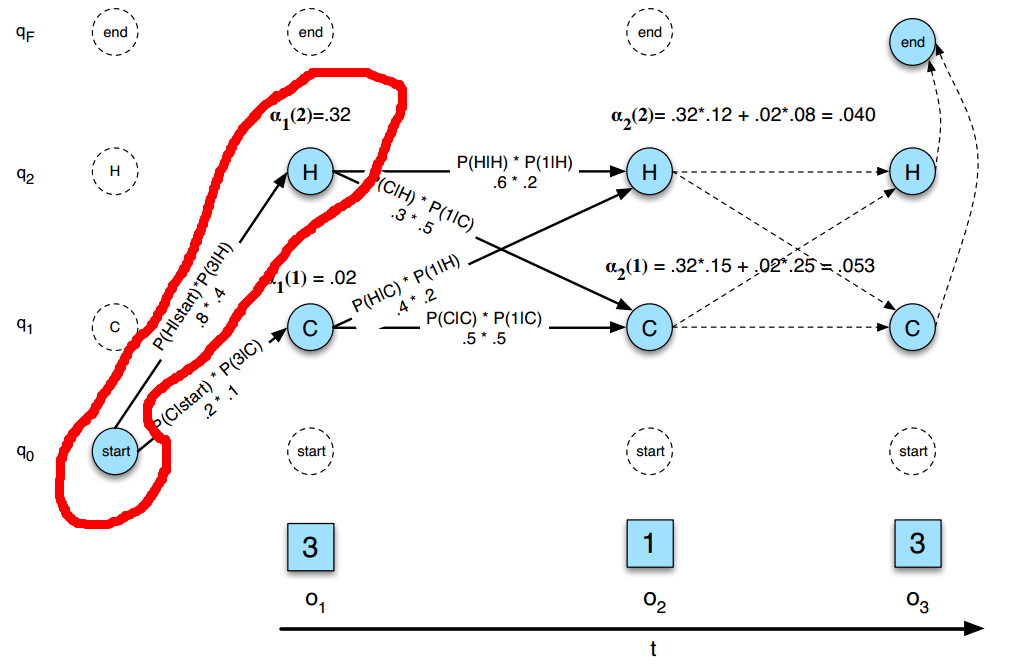
\includegraphics[width=4in,height=2.3in]{figures/the_forward_trellis_cells.png}
    \caption {\textbf{The forward trellis}}
  \end{figure}
%-------------------------------------------------------
\end{frame}
%-------------------------------------------------------

%-------------------------------------------------------
\subsection{Likelihood Computation: The Forward ALgorithm}
%-------------------------------------------------------
\begin{frame}{Hidden Markov Model}{Decoding: The Viterbi Algorithm}
%-------------------------------------------------------
    \begin{block}{Cells of the Forward algorithm trellis}
        Given as input an HMM $\lambda=(A,B)$ and a sequence of observations \
        $O={0_1,o_2,...,o_T}$ find the most probable sequence of states \
        $Q={q_1q_2q_3...q_T}$.
    \end{block}
\end{frame}
%-------------------------------------------------------

%-------------------------------------------------------
\subsection{Decoding: The Viterbi Algorithm}
%-------------------------------------------------------
\begin{frame}{Hidden Markov Model}{Decoding: The Viterbi Algorithm}
%-------------------------------------------------------
    For each possible hidden stat sequence, we could run the forward algorithm\
    and compute the likelihood of the observation sequence given that hidden \
    state sequence. Then we could choose the hidden state sequence with the \
    maximum observation likelihood.
\end{frame}
%-------------------------------------------------------

%-------------------------------------------------------
\begin{frame}{Hidden Markov Model}{Decoding: The Viterbi Algorithm}
%-------------------------------------------------------
    \begin{block}{Viterbi algorithm}
         \begin{equation}
            v_t(j) = max_{i=1}^{N}v_{t-1}a_{ij}b_j(o_t)
         \end{equation}
         \begin{itemize}
           \item $v_{t-1}(i)$ the previous Viterbi path probability from the \
                          previous time step.
           \item $a_{ij}$ the transition probability from previous state $q_i$ \
                          to current state $q_j$
           \item $b_j(o_t)$ the state observation likelihood of the\
                            observation symbol $o_t$ given the current state $j$
         \end{itemize}
    \end{block}
\end{frame}
%-------------------------------------------------------

%-------------------------------------------------------
\begin{frame}{Hidden Markov Model}{Decoding: The Viterbi Algorithm}
%-------------------------------------------------------
  \begin{figure}[h]
    \centering
    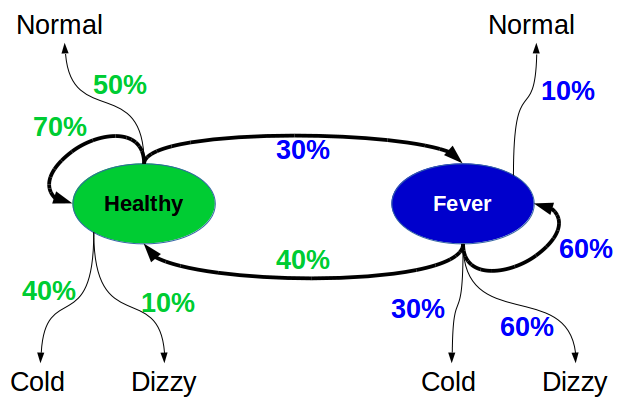
\includegraphics[width=4in,height=2.3in]{figures/doctor_example_01.png}
    \caption {\textbf{The Doctor and Patient example}}
  \end{figure}
\end{frame}
%-------------------------------------------------------

%-------------------------------------------------------
\begin{frame}{Hidden Markov Model}{Decoding: The Viterbi Algorithm}
%-------------------------------------------------------
  \begin{figure}[h]
    \centering
    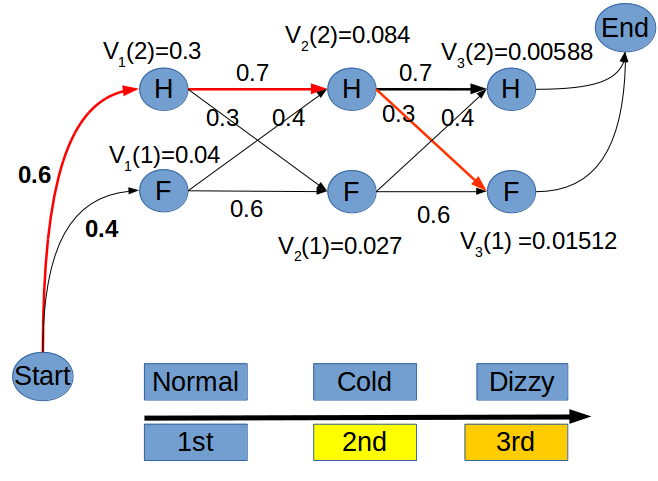
\includegraphics[width=4in,height=2.3in]{figures/doctor_example_02.png}
    \caption {\textbf{The Doctor and Patient example}}
  \end{figure}
\end{frame}
%-------------------------------------------------------

%-------------------------------------------------------
\subsection{Learning}
%-------------------------------------------------------
\begin{frame}{Hidden Markov Model}{Training}
%-------------------------------------------------------
    \begin{block}{Hidden Markov Model Training}
       Given an observation sequence $O$ and the sest of possible states in \
       the HMM, learn the HMM parameters A and B.
    \end{block}
    
    \begin{itemize}
       \item The input of a learning algorithm would be an unlabeled sequence \
             of observations $O$ and a vocabulary of potential hidden states \
             $Q$.
    \end{itemize}

\end{frame}
%-------------------------------------------------------

%-------------------------------------------------------
\subsection{Learning}
%-------------------------------------------------------
\begin{frame}{Hidden Markov Model}{Learning}
%-------------------------------------------------------
    \begin{block}{Training Algorithm}
        The standard algorithm for HMM training is the forward-backward, or \
        Baum-Welch algorithm which is a special case of the\
        Expectation-Maximization or EM algorithm.
    \end{block}
    \begin{block}{Training Algorithm}
        The algorithm is used for both transition probabilities A and the \
        emission probabilities B of the Hidden Markov Model.
    \end{block}
    \begin{block}{Training Algorithm}
        It works by computing an initial estimate for the probabilites, then \
        using those estimates to computing a better estimate, and so on, \
        iteratively improving the probabilities that it learns.
    \end{block}
\end{frame}
%-------------------------------------------------------

%-------------------------------------------------------
\begin{frame}{Hidden Markov Model}{Training: Example 6.3.1}
%-------------------------------------------------------
  \begin{figure}[h]
    \centering
    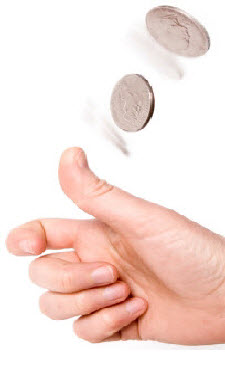
\includegraphics[width=4in,height=2.3in]{figures/coin_toss.jpg}
    \caption {\textbf{Example 6.3.1}}
  \end{figure}
\end{frame}
%-------------------------------------------------------

%-------------------------------------------------------
\begin{frame}{Hidden Markov Model}{Training: Example 6.3.1}
%-------------------------------------------------------
  \begin{figure}[h]
    \centering
    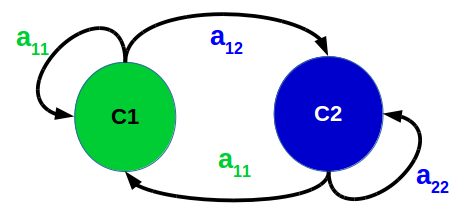
\includegraphics[width=4in,height=2.3in]{figures/toss_coin_example_01.png}
    \caption {\textbf{The Doctor and Patient example}}
  \end{figure}
\end{frame}
%-------------------------------------------------------

%-------------------------------------------------------
\begin{frame}{Hidden Markov Model}{Training: Example 6.3.1}
%-------------------------------------------------------
  \begin{figure}[h]
    \centering
    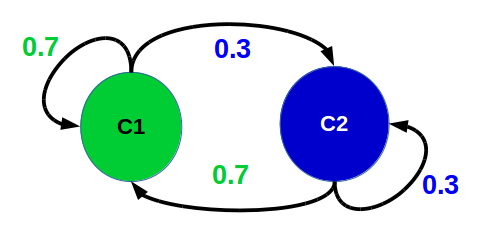
\includegraphics[width=4in,height=2.3in]{figures/toss_coin_example_02.png}
    \caption {\textbf{The Doctor and Patient example}}
  \end{figure}
\end{frame}
%-------------------------------------------------------

%-------------------------------------------------------
\begin{frame}{Hidden Markov Model}{Training: Example 6.3.1}
%-------------------------------------------------------
  \begin{figure}[h]
    \centering
    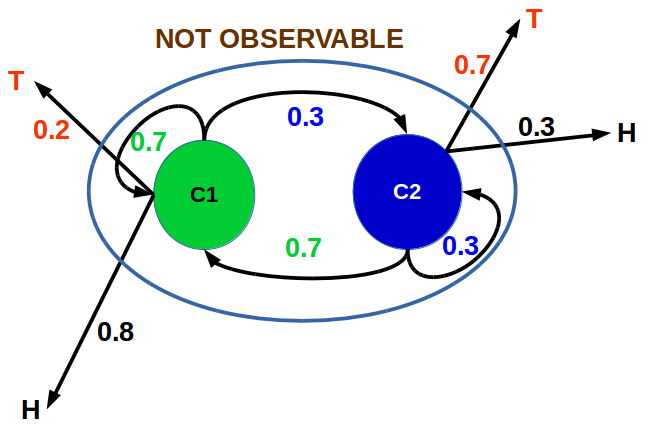
\includegraphics[width=4in,height=2.3in]{figures/toss_coin_example_03.png}
    \caption {\textbf{The Doctor and Patient example}}
  \end{figure}
\end{frame}
%-------------------------------------------------------

%-------------------------------------------------------
\begin{frame}{Hidden Markov Model}{Training: Example 6.3.1}
%-------------------------------------------------------
    \begin{block}{Source Code}
        A1 = [0.7 0.3;0.7 0.3];\\
        B1 = [0.8 0.3;0.2 0.7];\\
        pi1 = [0.7 0.3]';\\
         
        O = [1 1 1 2 1 1 1 1 2 1 1 1 1 2 2 1 1];
        
        [Pr1]=BWDoHMMst(pi1,A1,B1,O);
    \end{block}
\end{frame}
%-------------------------------------------------------

%
%%-------------------------------------------------------
%\subsection{Kidnapping Example cont.}
%%-------------------------------------------------------
%\begin{frame}{Hidden Markov Model}{Kidnapping Example cont.}
%%-------------------------------------------------------
%    Let go back again to \textbf{Kidnapping} example to discover how to apply\ 
%    Hidden Markov Model.
%  \begin{figure}[h]
%    \centering
%    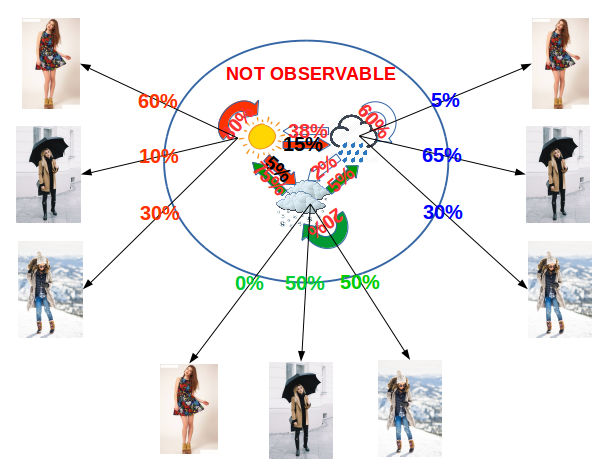
\includegraphics[width=3.5in,height=2in]{figures/kidnapping_example_model.png}
%    \caption {\textbf{Kidnapping Example}}
%  \end{figure}
%\end{frame}
%%-------------------------------------------------------
%
%%-------------------------------------------------------
%\begin{frame}{Hidden Markov Model}{Kidnapping Example cont.}
%%-------------------------------------------------------
%  \begin{figure}[h]
%    \centering
%    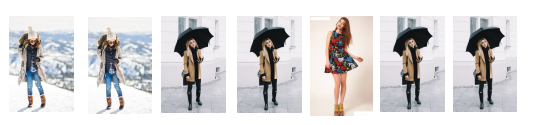
\includegraphics[width=3in,height=1in]{figures/kidnapping_example_02.png}
%    \caption {\textbf{What is the probability of this series?}}
%  \end{figure}
%\end{frame}
%%-------------------------------------------------------
%
%%-------------------------------------------------------
%\begin{frame}{Hidden Markov Model}{Kidnapping Example cont.}
%%-------------------------------------------------------
%  \textbf{Ingredients of "Kidnapping" Hidden Markov Model}
%  \fontsize{7.5}{10.5}
% {
%  \begin{itemize}
%     \item States: ${S_{sunny}, S_{rainy}, S_{snowy}}$
%     \item State transition probabilities: 
%            \begin{center}
%              \begin{tabular}{ |p{2cm}|p{1.2cm}|p{1.2cm}|p{1.2cm}| }
%                \hline
%                 \multicolumn{4}{|c|}{Weather Markov Model} \\
%                \hline
%                        & Sunny & Rainy & Snowy \\
%                \hline
%                     Sunny & 0.8  & 0.15 & 0.05\\
%                     Rainy & 0.38 & 0.6  & 0.02\\
%                     Snowy & 0.75 & 0.05 & 0.2\\
%                \hline
%              \end{tabular}
%              \end{center}
%      \item Distinct states: $\textbf{L} = \{C_1 = Short\ Skirt, C_2 = Umbrella, C_3 = Coat\}$
%      \item Observation sequences: $Y = \{y_1 = C_3, y_2 = C_3, y_3 = C_2, y_4 = C_2, y_5 = C_1, y_6 = C_2, y_7 = C_2\}$
%      \item Emission probability matrix:
%            \begin{center}
%              \begin{tabular}{ |p{2cm}|p{1.2cm}|p{1.2cm}|p{1.2cm}| }
%                \hline
%                 \multicolumn{4}{|c|}{Emission probability matrix} \\
%                \hline
%                        & Skirts & Umbrella & Coat \\
%                \hline
%                     Sunny & 0.6  & 0.1 & 0.3\\
%                     Rainy & 0.05 & 0.65  & 0.3\\
%                     Snowy & 0    & 0.5 & 0.5\\
%                \hline
%              \end{tabular}
%              \end{center}
%       \item Initial state distribution: $\pi = (0.7\ \ 0.25\ \ 0.05)$ 
%  \end{itemize}
% }
%\end{frame}
%%-------------------------------------------------------
%
%%-------------------------------------------------------
%\begin{frame}{Hidden Markov Model}{Kidnapping Example cont.}
%%-------------------------------------------------------
%    \textbf{\textcolor{red}{Are we missing something??????}}
%\end{frame}
%%-------------------------------------------------------
%
%%-------------------------------------------------------
%\begin{frame}{Hidden Markov Model}{Kidnapping Example cont.}
%%-------------------------------------------------------
%    To handle the example, we need to suppose that you was locked into the\
%    room is sunny and the caretaker wears short skirt. Hence:
%  \begin{itemize}
%      \item $\pi_{x_1}(1) = p(x_1 = S_{sunny}) = 0.7$\\
%      \item $b_{x_1}(y_1) =  0.6$
%  \end{itemize}
%\end{frame}
%%-------------------------------------------------------
%
%%-------------------------------------------------------
%\begin{frame}{Hidden Markov Model}{Kidnapping Example cont.}
%%-------------------------------------------------------
%   \begin{block}{Kidnapping Example Solution}
%      \begin{equation}
%         P(D) = [\pi_{x_1} \cdot b_{x_1}(y_1)] \cdot [a_{x_1,x_2} \cdot b_{x_2}(y_2)] \cdot [a_{x_3,x_2} \cdot b_{x_3}(y_3)]
%      \end{equation}
%  \ \ \ \ \ \ \ \ \ \ \ \ \ \ \ \ \ \ \ \ \ \ $= (0.7 \cdot 0.6) \cdot (0.15 \cdot 0.3) \cdot (0.05 \cdot 0.5)$
%   \end{block}
%\end{frame}
%%-------------------------------------------------------

{\1
\begin{frame}[plain,noframenumbering]
  \finalpage{Thanks for your attention}
\end{frame}}

\end{document}
